\documentclass{write_paper} 
\usepackage{amsmath}
\usepackage{ctex}
\usepackage{url}
%\usepackage{algorithm}
\usepackage{booktabs}
\usepackage{multirow}
\usepackage{algpseudocode}
\usepackage{subfigure}
\usepackage{epsfig}
\usepackage[utf8]{inputenc}
\usepackage[linesnumbered, ruled, vlined]{algorithm2e}
\usepackage{amsmath}
\usepackage{booktabs}
\usepackage{multirow}
\usepackage{wrapfig}  % 确保导言区引入该包
\usepackage{tikz}
\usepackage{fontspec}
\usetikzlibrary{positioning, arrows.meta}
\usepackage{caption}
\setmainfont{Segoe UI Emoji}  % Windows 推荐
% \setmainfont{Noto Color Emoji}  % Linux 推荐
 
 
\usepackage{siunitx}
  
\sisetup{group-separator={,}} % 千位分隔符


\usepackage[hidelinks]{hyperref}
\hypersetup{
  colorlinks=true,
  linkcolor=blue,
  filecolor=magenta,      
  urlcolor=blue,
  citecolor=blue,
}
\makeatletter
\@ifundefined{newblock}{\def\newblock{\hskip .11em plus .33em minus .07em}}{}
\makeatother

\usepackage{enumitem}
\makeatletter
\renewcommand\section{\@startsection {section}{1}{\z@}%
                                   {-1ex \@plus -1ex \@minus -.1ex}%
                                   {1 ex \@plus.1ex}%
                                   {\normalfont\large\bfseries}}
\renewcommand\subsection{\@startsection{subsection}{2}{\z@}%
                                     {-1ex\@plus -1ex \@minus -.1ex}%
                                     {1ex \@plus .1ex}%
                                     {\normalfont \normalsize \bfseries}}
\renewcommand\subsubsection{\@startsection{subsubsection}{3}{\z@}%
                                     {-1ex\@plus -1ex \@minus -.1ex}%
                                     {1ex \@plus .1ex}%
                                     {\normalfont\normalsize\bfseries}}
\makeatother

\renewcommand{\theARTICLETOP}{}
\usepackage{fancyhdr}
\pagestyle{fancy}
\fancyhf{}
\fancyhead[LE,RO]{}
\fancyhead[RE,LO]{\scriptsize{计算金融与仿真课程论文} }
\fancyfoot[CE,CO]{\leftmark}
\cfoot{\thepage}

\usepackage[T1]{fontenc}
\usepackage{palatino}

\OneAndAHalfSpacedXI
\usepackage{color}
\usepackage{soul}

\DeclareMathOperator{\E}{\mathbb{E}}
\DeclareMathOperator{\R}{\mathbb{R}}
\DeclareMathOperator{\B}{\mathbb{B}}
\DeclareMathOperator{\Z}{\mathbb{Z}}

%%-----------------------------------------
%% 将作者-年份改为数字制
\usepackage[numbers]{natbib}  % 关键:numbers选项
% \bibpunct{[}{]}{,}{n}{}{,}   % 若需要可自行指定标点
%%-----------------------------------------

% 如果之前有 \bibpunct 设置, 请注释掉或删除以免冲突
% \bibpunct[, ]{(}{)}{,}{a}{}{,}%  <-- 原先作者-年份制, 需要注释或删除

\TheoremsNumberedThrough
\EquationsNumberedThrough
\MANUSCRIPTNO{} 
\newtheorem{prop}{{Proposition}}
%\newtheorem{lemma}{{Lemma}}

%\renewcommand{\algorithmicrequire}{{Input:}}
%\renewcommand{\algorithmicensure}{{Output:}}

\newtheorem{implication}{\noindent{Implication}}

\newcommand{\YH}[1]{{\color{blue}#1}}
\newcommand{\JJ}[1]{{\color{black}#1}}
\newcommand{\eat}[1]{}
\usepackage{graphicx}
\usepackage{listings}
\usepackage{xcolor}  % 可选:定义颜色

\lstset{
  language=Python,             % 设置语言
  basicstyle=\ttfamily\tiny, % 基本字体风格
  numbers=left,               % 行号位置,可选 right 或 none
  numberstyle=\tiny,          % 行号字体
  keywordstyle=\color{blue},  % 关键字颜色
  commentstyle=\color{gray},  % 注释颜色
  stringstyle=\color{orange}, % 字符串颜色
  backgroundcolor=\color{white}, % 背景色
  frame=single,               % 添加边框,可选 shadowbox/double
  breaklines=true,            % 自动换行
  captionpos=b,               % 标题位置,b 或 t
  tabsize=4,                  % tab 宽度
  showstringspaces=false,     % 不显示字符串中的空格
}

\usepackage{endnotes}
\let\footnote=\endnote
\def\notesname{Endnotes}

\usepackage[symbol]{footmisc}
\renewcommand{\thefootnote}{\fnsymbol{footnote}}

\newcommand{\bs}[1]{\boldsymbol{#1}}
\newcommand{\ml}[1]{\mathcal{#1}}
\newcommand{\mb}[1]{\mathbb{#1}}

\begin{document}

% 整页垂直居中
\vspace*{\fill}

\begin{center}

    
\includegraphics[width=0.4\textwidth]{Figures/校徽.png}\\[1cm]
       \Huge \bfseries
      {计算金融与仿真}\\[0.5cm]
       \Huge \bfseries
      {课程论文}\\[2cm]
    
    \Large
    \begin{table}[htbp]
    \centering
    \Large
    \begin{tabular}{ll}
   {论文题目 }: & 计算金融与仿真 \\
   {学生姓名}: & 李晶晶 \quad 张璐 \quad 朱冯婧 \\
   {指导老师}: & 邓智斌 
    \end{tabular}
    \end{table}

    


\end{center}

\vspace*{\fill}
\newpage
\tableofcontents
\newpage




\section{投资组合选择介绍}


P2P借贷(peer-to-peer lending lending)是一种个人之间直接借贷的方式, 通过在线平台进行, 无需传统银行中介. 这种创新的融资方式提供了一个市场, 借款人可以向多个贷方申请贷款, 贷方可以选择为这些贷款提供全部或部分资金. 这一模式利用技术手段简化了借贷过程, 通常为借款人带来更低的利率, 同时为投资者提供更高的回报. 

目前, 全球几大平台主导着 P2P 借贷领域, 主要包括 LendingClub, Prosper 和 Funding Circle 等. 这类平台通过评估贷款项目和借款人的 FICO 分数, 贷款金额和期限, 借款人的资产, 债务状况, 就业类型等数据, 为每笔贷款提供风险评级. 其中, LendingClub 是美国最大的 P2P 借贷平台之一, 提供个人贷款和投资机会. 本文使用来自 LendingClub 的公共数据集(涵盖 2007--2018 年的贷款记录), 将贷款属性转化为违约概率作为后续建模依据. 

为了实现贷款投资组合的多元化, 投资者可依据自身的风险偏好从不同风险等级的贷款中进行选择. 与传统金融机构贷款不同, P2P 贷款中的每位个人投资者其可用于投资的资金较为有限. 因此, 如何在资金约束下, 基于借款人的风险特征评估潜在回报与风险, 选择合适的贷款项目, 并进行最优资金配置, 是 P2P 投资者亟需解决的问题. 

大量学者针对 P2P 网络贷款的投资组合优化问题开展了深入研究. Wan 等人将贷款投资组合决策转化为一个在特定时点下实现收益最大化与风险最小化的优化问题, 并引入混合治愈模型(mixture cure model,MCM)以提升投资效果, 构建实例驱动的模型对投资者的组合决策进行优化~\cite{wan2023hybrid}. Guo 等人则提出一种基于实例的 P2P 投资组合决策模型, 从风险最小角度出发, 利用 LendingClub 和 Prosper 数据集实现投资组合配置优化~\cite{guo2016instance}. Ajay 等人则将该问题转化为多目标优化模型, 在计算贷款相似度时将期望值框架与传统核方法结合, 优化结果优于既有模型\cite{byanjankar2021data}.

贷款投资组合优化(Loan Portfolio Optimization)与传统投资组合优化具有相似性, 但更关注与贷款相关的特定风险, 例如借款人信用评分, 贷款金额, 借款用途等因素引发的借款人风险, 违约风险以及利率波动风险. 优化目标是通过合理配置不同借款人贷款项目, 在控制风险的同时实现收益最大化. 

在风险量化方面, VaR(Value at Risk)与 CVaR(Conditional Value at Risk)被广泛用于衡量投资组合的风险水平. 其中, VaR 表示在置信水平 $\alpha$ 下, 金融资产或组合在未来特定持有期内的最大可能损失;而 CVaR 则刻画了超过 VaR 截止点的极端损失的期望, 即对尾部风险的加权平均, 是更稳健的风险衡量指标. 在贷款组合优化中, CVaR 能够帮助投资者更有效地控制整体尾部损失风险, 从而实现收益与风险的权衡优化. 




\section{模型建立}
\subsection{风险度量方法简介:VaR 与 CVaR}

在实际投资决策中,单纯追求期望收益往往难以满足风险控制的需要。尤其是在 P2P 贷款等高风险资产配置场景中,投资者更为关注潜在损失的严重程度及其发生概率。因此,在构建优化模型时,引入有效的风险度量工具显得尤为必要。本文主要采用两种广泛应用于金融风险管理领域的工具:\textbf{风险价值}(Value at Risk, VaR)与\textbf{条件风险价值}(Conditional Value at Risk, CVaR)。

\paragraph{VaR(Value at Risk)} 衡量在给定置信水平 $\beta$ 下,投资组合在未来某一时间段内的最大可能损失。若将投资组合损失视为随机变量 $L$,则其形式定义为:
\[
\text{VaR}_\beta(L) = \inf \left\{ \eta \in \mathbb{R} \mid \mathbb{P}(L \leq \eta) \geq \beta \right\},
\]
即在置信水平 $\beta$ 下,损失超过 $\text{VaR}_\beta$ 的概率不超过 $1 - \beta$。

\paragraph{CVaR(Conditional Value at Risk)} 则在 VaR 的基础上进一步刻画了尾部风险的严重程度,定义为在损失超过 VaR 的条件下的期望损失:
\[
\text{CVaR}_\beta(L) = \mathbb{E}[L \mid L \geq \text{VaR}_\beta(L)].
\]
与 VaR 相比,CVaR 更为保守,能够提供对极端损失更全面的评估,因而在面向风险厌恶型投资者的优化建模中具有更高的实用价值。

\subsection{模型设定与参数说明}

为系统性地构建贷款投资组合优化问题的数学模型,本文首先定义各类关键参数,如表~\ref{tab:parameters} 所示。该参数体系涵盖了贷款属性、投资者预算限制、风险容忍度约束、信用等级控制等方面,是后续模型构建的基础。

\begin{table}[htbp]
\centering
\caption{模型参数说明}
\label{tab:parameters}
\begin{tabular}{ll}
\toprule
参数符号 & 含义 \\
\midrule
$x_i$ & 决策变量,选择第 $i$ 个贷款时 $x_i = 1$,否则为 $0$ \\
$A_i$ & 第 $i$ 个贷款的申请金额 \\
$r_i$ & 第 $i$ 个贷款的年利率 \\
$P_i$ & 第 $i$ 个贷款的违约概率 \\
$B$ & 投资者可用的总预算 \\
$R_{\max}$ & 可接受的最大预期违约损失 \\
$G_k$ & 第 $k$ 类信用等级所包含的贷款集合 \\
$\alpha_k$ & 第 $k$ 类信用等级贷款可投资金额占比上限 \\
$m$ & 可选择的贷款项目数量上限(即 Top-$m$) \\
\bottomrule
\end{tabular}
\end{table}

\subsection{模型构建}

基于上述参数设定,本文提出三个层次递进的优化模型,以适应不同风险偏好与投资策略需求.首先,构建一个以期望收益最大化为核心目标的基本模型,适用于风险承受能力较高的投资者。该模型在满足预算、信用等级分散度、违约风险容忍度和项目数量等约束条件下,最大化组合的期望回款。
 

\begin{equation}
\begin{aligned}
\max_{x_i \in \{0,1\}} \quad & \sum_{i=1}^N x_i A_i  r_i(1 - P_i) \\
\text{s.t.} \quad
& \sum_{i=1}^N x_i A_i \le B, \\
& \sum_{i \in G_k} x_i A_i \le \alpha_k B, \quad \forall k, \\
& \sum_{i=1}^N x_i A_i P_i \le R_{\max}, \\
& \sum_{i=1}^N x_i \le m.
\end{aligned}
\label{eq:main_model}
\tag{P2P}
\end{equation}

该模型以期望收益最大化为核心目标,辅以预算、信用等级分散度、违约风险容忍度和项目数量的约束条件。适用于风险承受能力较高的投资者,其重点关注平均回报水平,对尾部风险的关注相对较弱。
 

为进一步控制极端损失发生的概率,引入 VaR 约束构建如下模型,
\begin{equation}
\begin{aligned}
\max_{x_i \in \{0,1\}} \quad & \sum_{i=1}^N x_i A_i  r_i(1 - P_i) \\
\text{s.t.} \quad
& \sum_{i=1}^N x_i A_i \le B, \\
& \sum_{i \in G_k} x_i A_i \le \alpha_k B, \quad \forall k, \\
& \sum_{i=1}^N x_i A_i \cdot \tilde{P}_i^{(s)} - \eta \le \mathcal{M} z_s, \quad \forall s = 1,\dots,S, \\
& \sum_{s=1}^S z_s \le (1 - \beta) S, \\
& \sum_{i=1}^N x_i \le m, \\
& z_s \in \{0,1\}, \quad \eta \in \mathbb{R}.
\end{aligned}
\label{eq:var_model}
\tag{P2P-VaR}
\end{equation}

其中,$\tilde{P}_i^{(s)}$ 表示第 $s$ 个情景下第 $i$ 个贷款的违约概率估计值,$z_s$ 为辅助变量,$\mathcal{M}$ 为足够大的常数。该模型通过场景模拟方式,限制损失超出阈值 $\eta$ 的情景数量,从而降低极端损失发生概率,适用于注重稳健性的投资者。
 

在控制极端损失概率的基础上,进一步引入 CVaR 约束,以衡量尾部损失的平均程度,构建如下优化模型,

\begin{equation}
\begin{aligned}
\max_{x_i \in \{0,1\}} \quad & \sum_{i=1}^N x_i A_i r_i(1 - P_i) \\
\text{s.t.} \quad
& \sum_{i=1}^N x_i A_i \le B, \\
& \sum_{i \in G_k} x_i A_i \le \alpha_k B, \quad \forall k, \\
& \xi_s \ge \sum_{i=1}^N x_i A_i \cdot \tilde{P}_i^{(s)} - \eta, \quad \forall s = 1,\dots,S, \\
& \eta + \frac{1}{S(1 - \beta)} \sum_{s=1}^S \xi_s \le \text{CVaR}_{\max}, \\
& \sum_{i=1}^N x_i \le m, \\
& \xi_s \ge 0, \quad \eta \in \mathbb{R}.
\end{aligned}
\label{eq:cvar_model}
\tag{P2P-CVaR}
\end{equation}

其中,$\xi_s$ 表示每个情景中损失超出 VaR 水平的部分,CVaR 约束确保尾部平均损失不超过上限 $\text{CVaR}_{\max}$。该模型适用于风险厌恶程度更高、对极端事件高度敏感的投资者,进一步增强了组合的鲁棒性与稳定性。

 

综上所述,本文构建了一个由浅入深的贷款投资优化模型体系:模型~\eqref{eq:main_model} 聚焦期望收益最大化,模型~\eqref{eq:var_model} 引入 VaR 约束以控制极端损失的概率,模型~\eqref{eq:cvar_model} 则进一步施加 CVaR 约束以控制尾部损失的严重程度。投资者可依据自身的风险偏好与收益目标,灵活选用相应模型,实现个性化的最优投资决策方案。

\section{算法设计}
\subsection{粒子群优化算法(PSO)}

粒子群优化算法(Particle Swarm Optimization, PSO)是一种基于群体智能的随机优化方法,由 Kennedy 和 Eberhart 于 1995 年提出~\cite{kennedy1995particle}。该算法受鸟群觅食行为的启发,模拟粒子在解空间中基于个体经验与群体经验协同搜索最优解的过程。

在 PSO 中,每个粒子代表一个潜在解,其状态由位置与速度两个向量描述。粒子在搜索过程中根据个体历史最优位置(Personal Best, $pbest$)和群体历史最优位置(Global Best, $gbest$)共同指导其移动方向与速度调整。具体的更新公式如下:
\[
\begin{aligned}
v_i^{(t+1)} &= w \cdot v_i^{(t)} + c_1 \cdot r_1 \cdot (pbest_i - x_i^{(t)}) + c_2 \cdot r_2 \cdot (gbest - x_i^{(t)}), \\
x_i^{(t+1)} &= x_i^{(t)} + v_i^{(t+1)},
\end{aligned}
\]
其中,$x_i^{(t)}$ 与 $v_i^{(t)}$ 分别表示第 $i$ 个粒子在第 $t$ 代的位置信息与速度;$w$ 为惯性权重,控制粒子搜索的稳定性;$c_1$ 和 $c_2$ 分别为个体学习因子与群体学习因子;$r_1$ 和 $r_2$ 为服从 $[0,1]$ 区间均匀分布的随机数,用于增强算法的随机探索能力。

PSO 算法的优点在于结构简单、参数少、全局搜索能力强,尤其适用于复杂非凸、不可导甚至离散的组合优化问题。但其缺点是缺乏精确性与最优性保证,通常作为启发式方法用于生成可行解或局部最优解。

\subsection{PSO 与 Gurobi 联合优化框架}
\vspace{-1ex}

\begin{wrapfigure}{l}{0.45\textwidth}
\vspace{-1ex}
\centering
\begin{tikzpicture}[node distance=1.5cm, every node/.style={font=\small}]
  \tikzstyle{startstop} = [rectangle, rounded corners, minimum width=4cm, minimum height=0.8cm, text centered, draw=black, fill=blue!10]
  \tikzstyle{process} = [rectangle, minimum width=4cm, minimum height=0.8cm, text centered, draw=black, fill=gray!10]
  \tikzstyle{arrow} = [thick,->,>=stealth]

  \node (start) [startstop] {🚀 开始:初始化参数};
  \node (pso) [process, below of=start] {🐦 PSO 粒子群搜索};
  \node (decode) [process, below of=pso] {🧠 解码粒子};
  \node (select) [process, below of=decode] {🌟 选取最优解};
  \node (gurobi) [process, below of=select] {🧮 Gurobi 求解};
  \node (end) [startstop, below of=gurobi] {📊 输出结果};

  \draw [arrow] (start) -- (pso);
  \draw [arrow] (pso) -- (decode);
  \draw [arrow] (decode) -- (select);
  \draw [arrow] (select) -- (gurobi);
  \draw [arrow] (gurobi) -- (end);
\end{tikzpicture}
\caption{PSO 与 Gurobi 联合优化框架}
\label{fig:framework}
\vspace{-1ex}
\end{wrapfigure}

在本研究中,我们结合粒子群优化算法的全局搜索能力与 Gurobi 求解器的精确优化能力,构建了一个两阶段优化框架,如图~\ref{fig:framework} 所示。该方法首先利用 PSO 在全局搜索空间中生成可行解,然后通过 Gurobi 进一步精细求解,实现粗定位与精优化的协同融合。

第一阶段为粒子群优化(PSO),其通过初始化种群并迭代演化,在可行域内快速定位高质量解空间。第二阶段将 PSO 输出的最优候选解作为 warm-start 初始化输入至 Gurobi,执行整数规划模型的精确求解,从而得到满足所有约束条件的最优解或近似最优解。

该框架在实际运行中表现出良好的效率与稳定性:PSO 能在大规模组合空间中迅速收敛至高质量区域,Gurobi 则在此基础上进一步提升解的精度。两者配合弥补了启发式算法的全局性与精确算法的局部性之间的差距,体现了“启发探索 + 精确强化”的优化策略。

为提升整体求解效率,我们还设置了如下机制:
\begin{itemize}
    \item 基于评分的粒子位置解码机制,将实数粒子映射为可行的 0-1 决策向量;
    \item 引入精英保留策略,防止 Gurobi 从劣解出发;
    \item 在 PSO 阶段提前剔除低效粒子,减少冗余迭代;
    \item 设置 Gurobi 的时间限制与 MIPGap 约束,以平衡解质量与计算代价。
\end{itemize}

综上,PSO+Gurobi 联合优化框架充分整合了群体智能的搜索优势与数学规划的求解精度,为解决复杂约束下的贷款投资组合优化问题提供了高效、鲁棒的技术支持。
\section{案例研究}
\label{sec:case_study}
\subsection{数据集描述}

\label{subsec:dataset_description}

本研究使用的数据集来自 Lending Club 平台, 原始数据由 Kaggle 网站\url{https://www.kaggle.com/datasets/wordsforthewise/lending-club}公开提供. Lending Club 是美国最大的网络借贷平台之一, 提供了详尽的个人借款申请及其还款情况的数据, 广泛应用于学术界和工业界进行信贷风险评估, 违约预测及投资组合优化等研究. 

该数据集包含了从 2007 年至 2018 年的借款记录, 共计数百万条样本. 每条记录对应一笔贷款申请, 涵盖了包括贷款金额, 利率, 借款人信用等级, 债务收入比, 贷款期限, 还款状态, 就业年限, 收入, 地址状态, 房屋所有权, FICO 评分区间等在内的多维度信息. 

在本研究中, 我们主要筛选并保留10种变量用于建模分析,如表\ref{tab:dataset_variables}所示. 这些变量涵盖了借款人的基本信息, 贷款合同的核心条款以及还款状态等关键信息, 为后续的风险评估与投资组合优化提供了必要的数据基础.
\begin{table}[htbp]
\centering
\caption{建模所用主要变量说明}
\label{tab:dataset_variables}
\begin{tabular}{ll}
\toprule
变量名称 & 含义说明 \\
\midrule
\texttt{loan\_amnt} & 借款人申请的贷款金额,对应模型中的 $A_i$ \\
\texttt{int\_rate} & 借款合同中约定的年利率,用于计算收益率 $r_i$ \\
\texttt{grade} & 借款人信用等级(A 至 G),用于构建信用等级集合 $G_k$ \\
\texttt{loan\_status} & 实际贷款还款状态(如 Fully Paid, Charged Off),用于推断违约情况 \\
\texttt{annual\_inc} & 借款人年收入,用于辅助风险刻画 \\
\texttt{dti} & 债务收入比(Debt-to-Income Ratio),用于增强风险特征描述 \\
\texttt{term} & 贷款期限(如 36 months 或 60 months) \\
\texttt{emp\_length} & 借款人工作年限 \\
\texttt{addr\_state} & 借款人所在州(美国各州) \\
\texttt{fico\_range\_high} & 借款人 FICO 信用评分上限,用于量化信用水平 \\
\texttt{fico\_range\_low} & 借款人 FICO 信用评分下限,用于量化信用水平 \\
\bottomrule
\end{tabular}
\end{table}
 

为了满足模型中对违约概率 $P_i$ 的需求, 使用机器学习预测违约概率作为后续优化模型的输入. 具体方法将在后续章节详细介绍.

此外, 为模拟贷款违约的风险场景, 我们以借款人的信用等级, FICO评分和历史违约频率为依据, 构建了 $S$ 个 Monte Carlo 风险场景, 用于后续 CVaR 优化模型的风险评估. 

通过上述数据处理步骤, 最终形成了一个结构规范, 信息完备, 适用于组合优化问题的数据集, 为后续实证分析与建模提供了坚实的数据基础. 

\begin{table}[htbp]
\centering
\caption{三类投资优化模型的主要参数设置}
\begin{tabular}{lll}
\toprule
 {参数符号} &{含义} &{适用模型} \\
\midrule
$B$ & 投资总预算,$1 \times 10^8$ 元 & 全部 \\
$m$ & 最多选择的贷款数量(Top-$m$),5000 & 全部 \\
$P_i$ & 贷款 $i$ 的违约概率,$P_i \in [0, 1]$ & 全部 \\
$R_{\max}$ & 风险容忍值上限,$1.5 \times 10^7$ 元 & 全部 \\
$\text{CVaR}_{\max}$ & 期望风险容忍值上限,$1.5 \times 10^7$ 元 & CVaR\\
$\beta$ & 置信水平(VaR、CVaR),0.95 & VaR ,CVaR\\
$\eta$ & VaR临界值(上界),动态变量 & VaR ,CVaR\\
$S$ & 蒙特卡洛模拟场景数量,1000 & VaR ,CVaR\\
$\alpha_k$ & 信用等级比例上限 & 全部\\
& \quad A: 40\%, B: 30\%, C: 20\%, D: 10\%, E: 5\%, F: 2\%, G: 1\% & \\
$pop\_size$ & 粒子群算法种群规模,30 & PSO  \\
$max\_iter$ & 粒子群最大迭代次数,100 & PSO  \\
$(w, c_1, c_2)$ & PSO 参数设置:$w=0.7$, $c_1=c_2=1.5$ & PSO  \\
\bottomrule
\end{tabular}
\label{tab:three-model-params}
\end{table}
\subsection{使用机器学习预测违约概率 $P_i$}
\label{subsec:predict_p_i}

尽管本研究使用的数据集中所有贷款均已获得实际资助, 但在资金有限, 需进行优选配置的情境下, 我们仍需要对这些已发放贷款的还款风险进行再评估. 为此, 我们引入机器学习方法, 对每笔贷款的未来违约概率 $P_i$ 进行预测建模, 以作为后续优化模型中的风险输入参数. 

 
预测函数的目标是:对于每笔已发放贷款 $i$, 根据其已知特征向量 $\mathbf{x}_i$, 估计其在未来发生违约的概率 $P_i = \mathbb{P}(y_i = 1 \mid \mathbf{x}_i)$. 其中, $y_i=1$ 表示贷款最终发生违约(如状态为 \texttt{Charged Off}), $y_i=0$ 表示贷款最终还清(如状态为 \texttt{Fully Paid}). 

 
我们基于借款人基本属性, 贷款合同信息以及信用评级等信息构建预测特征集, 涵盖表~\ref{tab:dataset_variables} 中列出的变量。

 
考虑到目标变量仍是二元状态(违约 / 未违约), 我们采用监督学习的二分类方法进行建模. 尝试的模型包括逻辑回归(Logistic Regression), 随机森林(Random Forest), 梯度提升树(GBDT), 极端梯度提升(XGBoost)等. 

由于样本中违约样本占比相对较小, 我们在训练过程中采用类别加权, 欠采样等方式处理类别不平衡问题. 

 

我们将全部已发放贷款随机划分为训练集(70\%)与测试集(30\%), 使用交叉验证调优参数, 并基于测试集评估模型表现. 评价指标包括准确率(Accuracy), AUC 值(Area Under the ROC Curve), F1 分数等. 

最终, 我们选择 AUC 表现最优的模型用于对所有贷款样本生成违约概率预测值 $\hat{P}_i$, 作为后续优化模型中的输入. 
 
虽然原始数据中每笔贷款都已实际放款, 但我们的建模任务是为现实中的“再选择”提供依据. 即在预算受限, 资源不足时, 如何在这些真实已放款的贷款中优先挑选违约概率低, 预期收益高的子集, 构建一个更稳健的投资组合. 因此, $\hat{P}_i$ 的预测并非用于决定放款与否, 而是作为组合优化的“风险估计量”, 用于构建期望收益与 CVaR 等风险指标. 
\subsection{三类优化模型的构建与求解}
为了刻画贷款组合的期望收益与风险约束之间的权衡,本文依次构建了三个层次递进的优化模型。首先,算法~\ref{alg:primal_model} 基于期望损失约束进行建模,在预算、人数与信用等级结构等限制条件下,最大化组合的期望回款,适用于风险偏好较高的情境。为进一步控制尾部风险,算法~\ref{alg:var_model} 引入 VaR约束,通过模拟场景下的分位损失限制组合在置信水平内的最大损失。考虑到 VaR 仅刻画极端事件的临界值,不反映其之后的损失程度,算法~\ref{alg:cvar_model} 进一步纳入 CVaR约束,以捕捉尾部分布的平均损失。三者构成由“平均控制”到“尾部控制”的风险建模体系,为投资者在不同风险偏好下提供灵活的策略选择。
\label{subsec:model_solving}
 \begin{algorithm}[htbp]  \footnotesize
\caption{原始模型:最大化期望回款}
\label{alg:primal_model}
\KwIn{贷款数据集:$A_i$, $r_i$, $P_i$, $grade_i$}
\KwOut{最优组合 $x_i \in \{0,1\}$}

\textbf{1. 数据处理:} \\
计算收益 $profit_i = A_i \cdot r_i \cdot (1 - P_i)$ \\
构造信用等级分组与比例约束 $\alpha_k$

\textbf{2. 参数设定:} \\
总预算 $B$、人数上限 $m$、期望损失上限 $R_{\max}$

\textbf{3. 构建模型:} \\
最大化目标函数 $\sum_i x_i \cdot profit_i$ \\
约束包括:
\begin{itemize}
  \item 预算:$\sum_i x_i A_i \leq B$
  \item 信用等级占比:$\sum_{i \in \text{grade}_k} x_i A_i \leq \alpha_k B$
  \item 期望损失:$\sum_i x_i A_i P_i \leq R_{\max}$
  \item 投资数量限制:$\sum_i x_i \leq m$
\end{itemize}

\textbf{4. 求解与输出:} \\
调用 Gurobi 优化器,输出最优解、收益、投资额和等级统计结果
\end{algorithm}



 \begin{algorithm}[htbp]  \footnotesize
\caption{VaR 模型:风险控制下的收益最大化}
\label{alg:var_model}
\KwIn{贷款数据集:$A_i$, $r_i$, $P_i$, $grade_i$}
\KwOut{最优组合 $x_i \in \{0,1\}$,VaR 风险值 $\eta$}

\textbf{1. 数据与场景构造:} \\
计算 $profit_i$,模拟 $S$ 个违约场景 $L_{i,s} \sim \text{Bernoulli}(P_i)$

\textbf{2. 参数设置:} \\
预算 $B$、人数上限 $m$、VaR 置信水平 $\beta$、上界 $\eta_{\max}$

\textbf{3. 粒子群优化(PSO):} \\
初始化解与群体;定义适应度函数 \\
判断组合是否满足:
\begin{itemize}
  \item 投资约束与等级比例限制
  \item 期望损失限制:$\sum_i x_i A_i P_i \leq R_{\max}$
  \item VaR 约束:第 $\alpha$ 分位损失 $\eta \leq \eta_{\max}$
\end{itemize}
目标为最大化 $\sum_i x_i profit_i - \text{惩罚项}$

\textbf{4. Gurobi 精确建模:} \\
引入变量 $x_i$, $\eta$, $z_s$,线性化 VaR 表达:
\(
\sum_i x_i A_i L_{i,s} - \eta \leq M \cdot z_s,\quad \sum_s z_s \leq \alpha S
\)
以PSO解初始化,最大化期望收益
\end{algorithm}



 \begin{algorithm}[htbp]  \footnotesize
\caption{基于CVaR约束的贷款组合优化}
\label{alg:cvar_model}
\KwIn{贷款数据集:$A_i$(金额),$r_i$(利率),$P_i$(违约概率),信用等级 $grade_i$}
\KwOut{最优组合 $x_i \in \{0,1\}$,CVaR 风险值}

\textbf{1. 数据处理与模拟:} \\
清洗数据,构造收益 $profit_i = A_i \cdot r_i \cdot (1 - P_i)$ \\
模拟 $S$ 个场景的违约矩阵 $L_{i,s} \sim \text{Bernoulli}(P_i)$

\textbf{2. 参数设置:} \\
设定预算 $B$,人数限制 $m$,置信水平 $\beta$,CVaR 上限 $R_{\max}$,粒子群参数 $(w, c_1, c_2)$

\textbf{3. 粒子群初始化与适应度函数:} \\
初始化种群与启发式解 \\
评估函数为:
\(
\text{CVaR}_\beta = \eta + \frac{1}{(1-\beta)S} \sum_{s=1}^S \max(0, \ell_s - \eta)
\)
其中 $\ell_s = \sum_i x_i A_i L_{i,s}$ \\
若满足 $\text{CVaR}_\beta \leq R_{\max}$,最大化 $\sum_i x_i profit_i + \text{奖励项}$

\textbf{4. PSO 迭代寻优:} \\
按惯性与个体/全局最优更新粒子,sigmoid 映射生成 $x_i$ 的选取概率

\textbf{5. Gurobi 精确求解:} \\
构建混合整数模型,定义变量 $x_i$, $\eta$, $\xi_s$ \\
约束包括预算、人数、等级比例、期望损失和 CVaR 表达:
\(
\xi_s \geq \sum_i x_i A_i L_{i,s} - \eta,\quad \eta + \frac{1}{(1-\beta)S} \sum_s \xi_s \leq R_{\max}
\)
以 PSO 解初始化,最大化期望收益
\end{algorithm}

\subsection{结果分析}
\label{subsec:result_analysis}


表~\ref{tab:result-comparison} 汇总了三种优化模型(即模型~\ref{eq:main_model}、模型~\ref{eq:var_model} 和模型~\ref{eq:cvar_model})在不同求解方法(Gurobi 与 PSO)下的结果表现,包括投资组合期望收益、所选中贷款数量以及 VaR 与 CVaR 上界等关键指标。整体来看,模型~\ref{eq:main_model} 所对应的 Gurobi 解获得了最高的期望收益(约为 759 万元),但未设置任何风险控制约束;相比之下,引入 VaR 与 CVaR 限制的模型虽在期望收益上有所让步,但显著降低了尾部风险和潜在损失的波动性,体现了优化目标对结果结构的实质性影响。
\begin{table}[htbp]
\centering
\caption{不同优化模型下的结果比较}
\label{tab:result-comparison}
\begin{tabular}{llllSSS}
\toprule
模型类型 & 方法 & 选中人数 & 投资组合期望收益 & {VaR 上界} & {CVaR 上界} \\
\midrule
\ref{eq:main_model}& Gurobi & 5000 & \textcolor{red}{\sisetup{group-separator={,}}\num{7596540.84}} & {--} & {--} \\
\midrule
\ref{eq:var_model}& PSO & 5000 & \num{7016573.73} & \num{36698075.00} & {--} \\
& Gurobi & 4157 & \textcolor{red}{\num{4803258.84}} & \num{16507725.00} & {--} \\
\midrule
\ref{eq:cvar_model} & PSO & 5000 & \num{7016573.73} & {--} & \num{36698075.00} \\
& Gurobi & 4347 & \textcolor{red}{\num{4774801.27}} & {--} & \num{14997692.00} \\
\bottomrule
\end{tabular}
\end{table}

图~\ref{fig:combined_results} 展示了三种模型下所选贷款在违约概率与年利率两个维度上的联合分布情况。图中每一个圆点表示一个利率-违约率组合,其大小和颜色深度反映了该组合中贷款样本的数量。可以观察到,不同模型在风险收益空间中的选择策略存在显著差异:模型~\ref{eq:main_model} 倾向于选取中等利率和中低违约概率的贷款,以获取较高的平均回报;模型~\ref{eq:var_model} 在控制尾部风险的基础上,更倾向于选择低违约率但利率略高的贷款;而模型~\ref{eq:cvar_model} 明显偏好低利率、低违约率的贷款组合,以牺牲部分收益换取更强的风险规避能力,表现出显著的保守投资取向。

\begin{figure}[htbp]
\centering
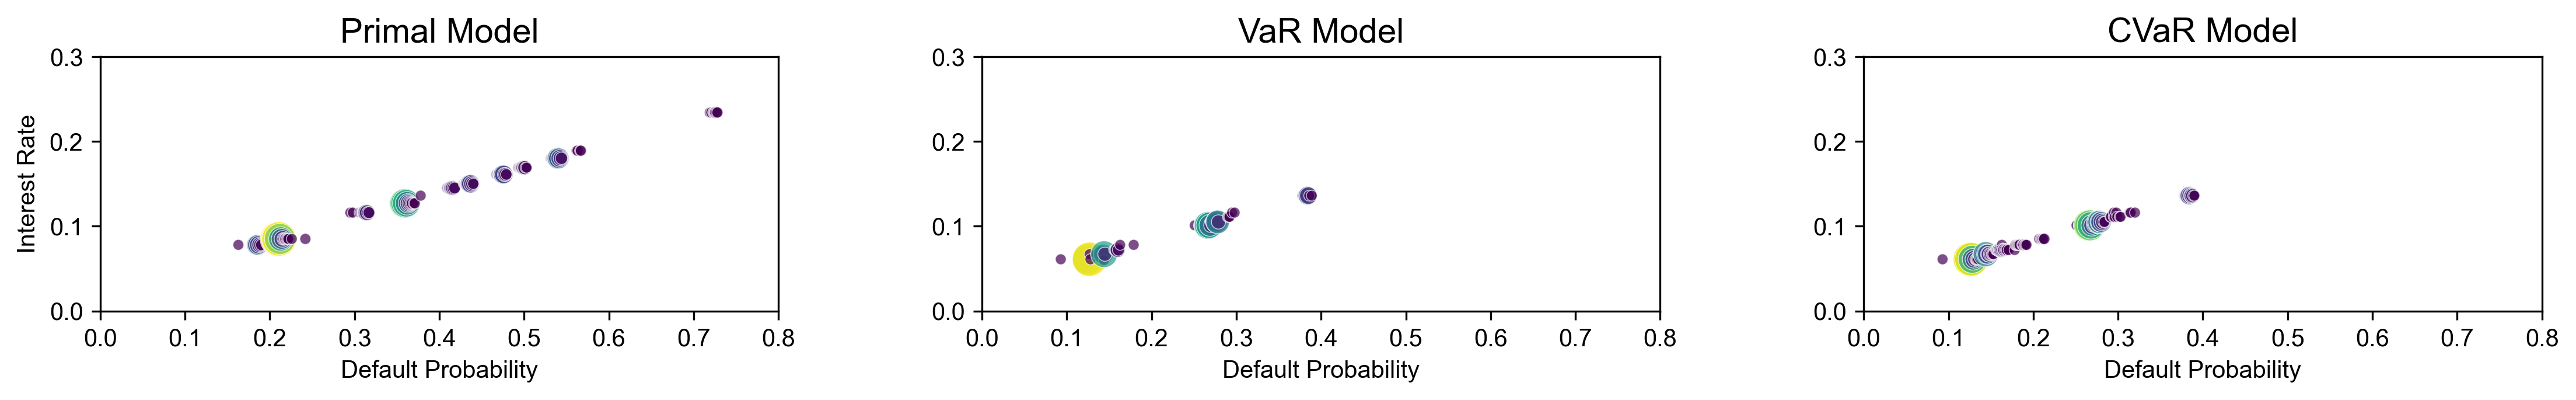
\includegraphics[width=\textwidth]{Figures/model_comparison_scatter.png}
\caption{三类模型下贷款样本在违约率与利率维度的联合分布}
\label{fig:combined_results}
\end{figure}

进一步地,图~\ref{fig:boxplot_comparison} 以箱线图形式从两个维度刻画了三类模型所选贷款的特征分布。子图~\ref{fig:expected_profit_boxplot} 显示的是期望收益分布,反映在不同模型下,单笔贷款所对应的收益分布情况。可以看出,模型~\ref{eq:main_model} 拥有最高的收益中位数,同时波动性也最大,存在若干极端高回报贷款;模型~\ref{eq:var_model} 的期望收益分布相对收敛,尾部风险有所缓释;而模型~\ref{eq:cvar_model} 则在剔除高风险高回报贷款的基础上,整体收益显著下降,但分布更为集中,进一步验证其稳健性取向。

子图~\ref{fig:loan_amount_boxplot} 展示了三种模型下贷款金额的分布情况。结果表明,模型~\ref{eq:main_model} 与模型~\ref{eq:var_model} 倾向于选取金额较大的贷款,前者甚至包含若干高达几十万元的大额贷款;相比之下,模型~\ref{eq:cvar_model} 更偏向于选择金额较小的贷款组合,通过限制潜在单笔损失规模,进一步实现整体风险的压缩。

\begin{figure}[htbp]
\centering
\subfigure[期望收益分布]{
  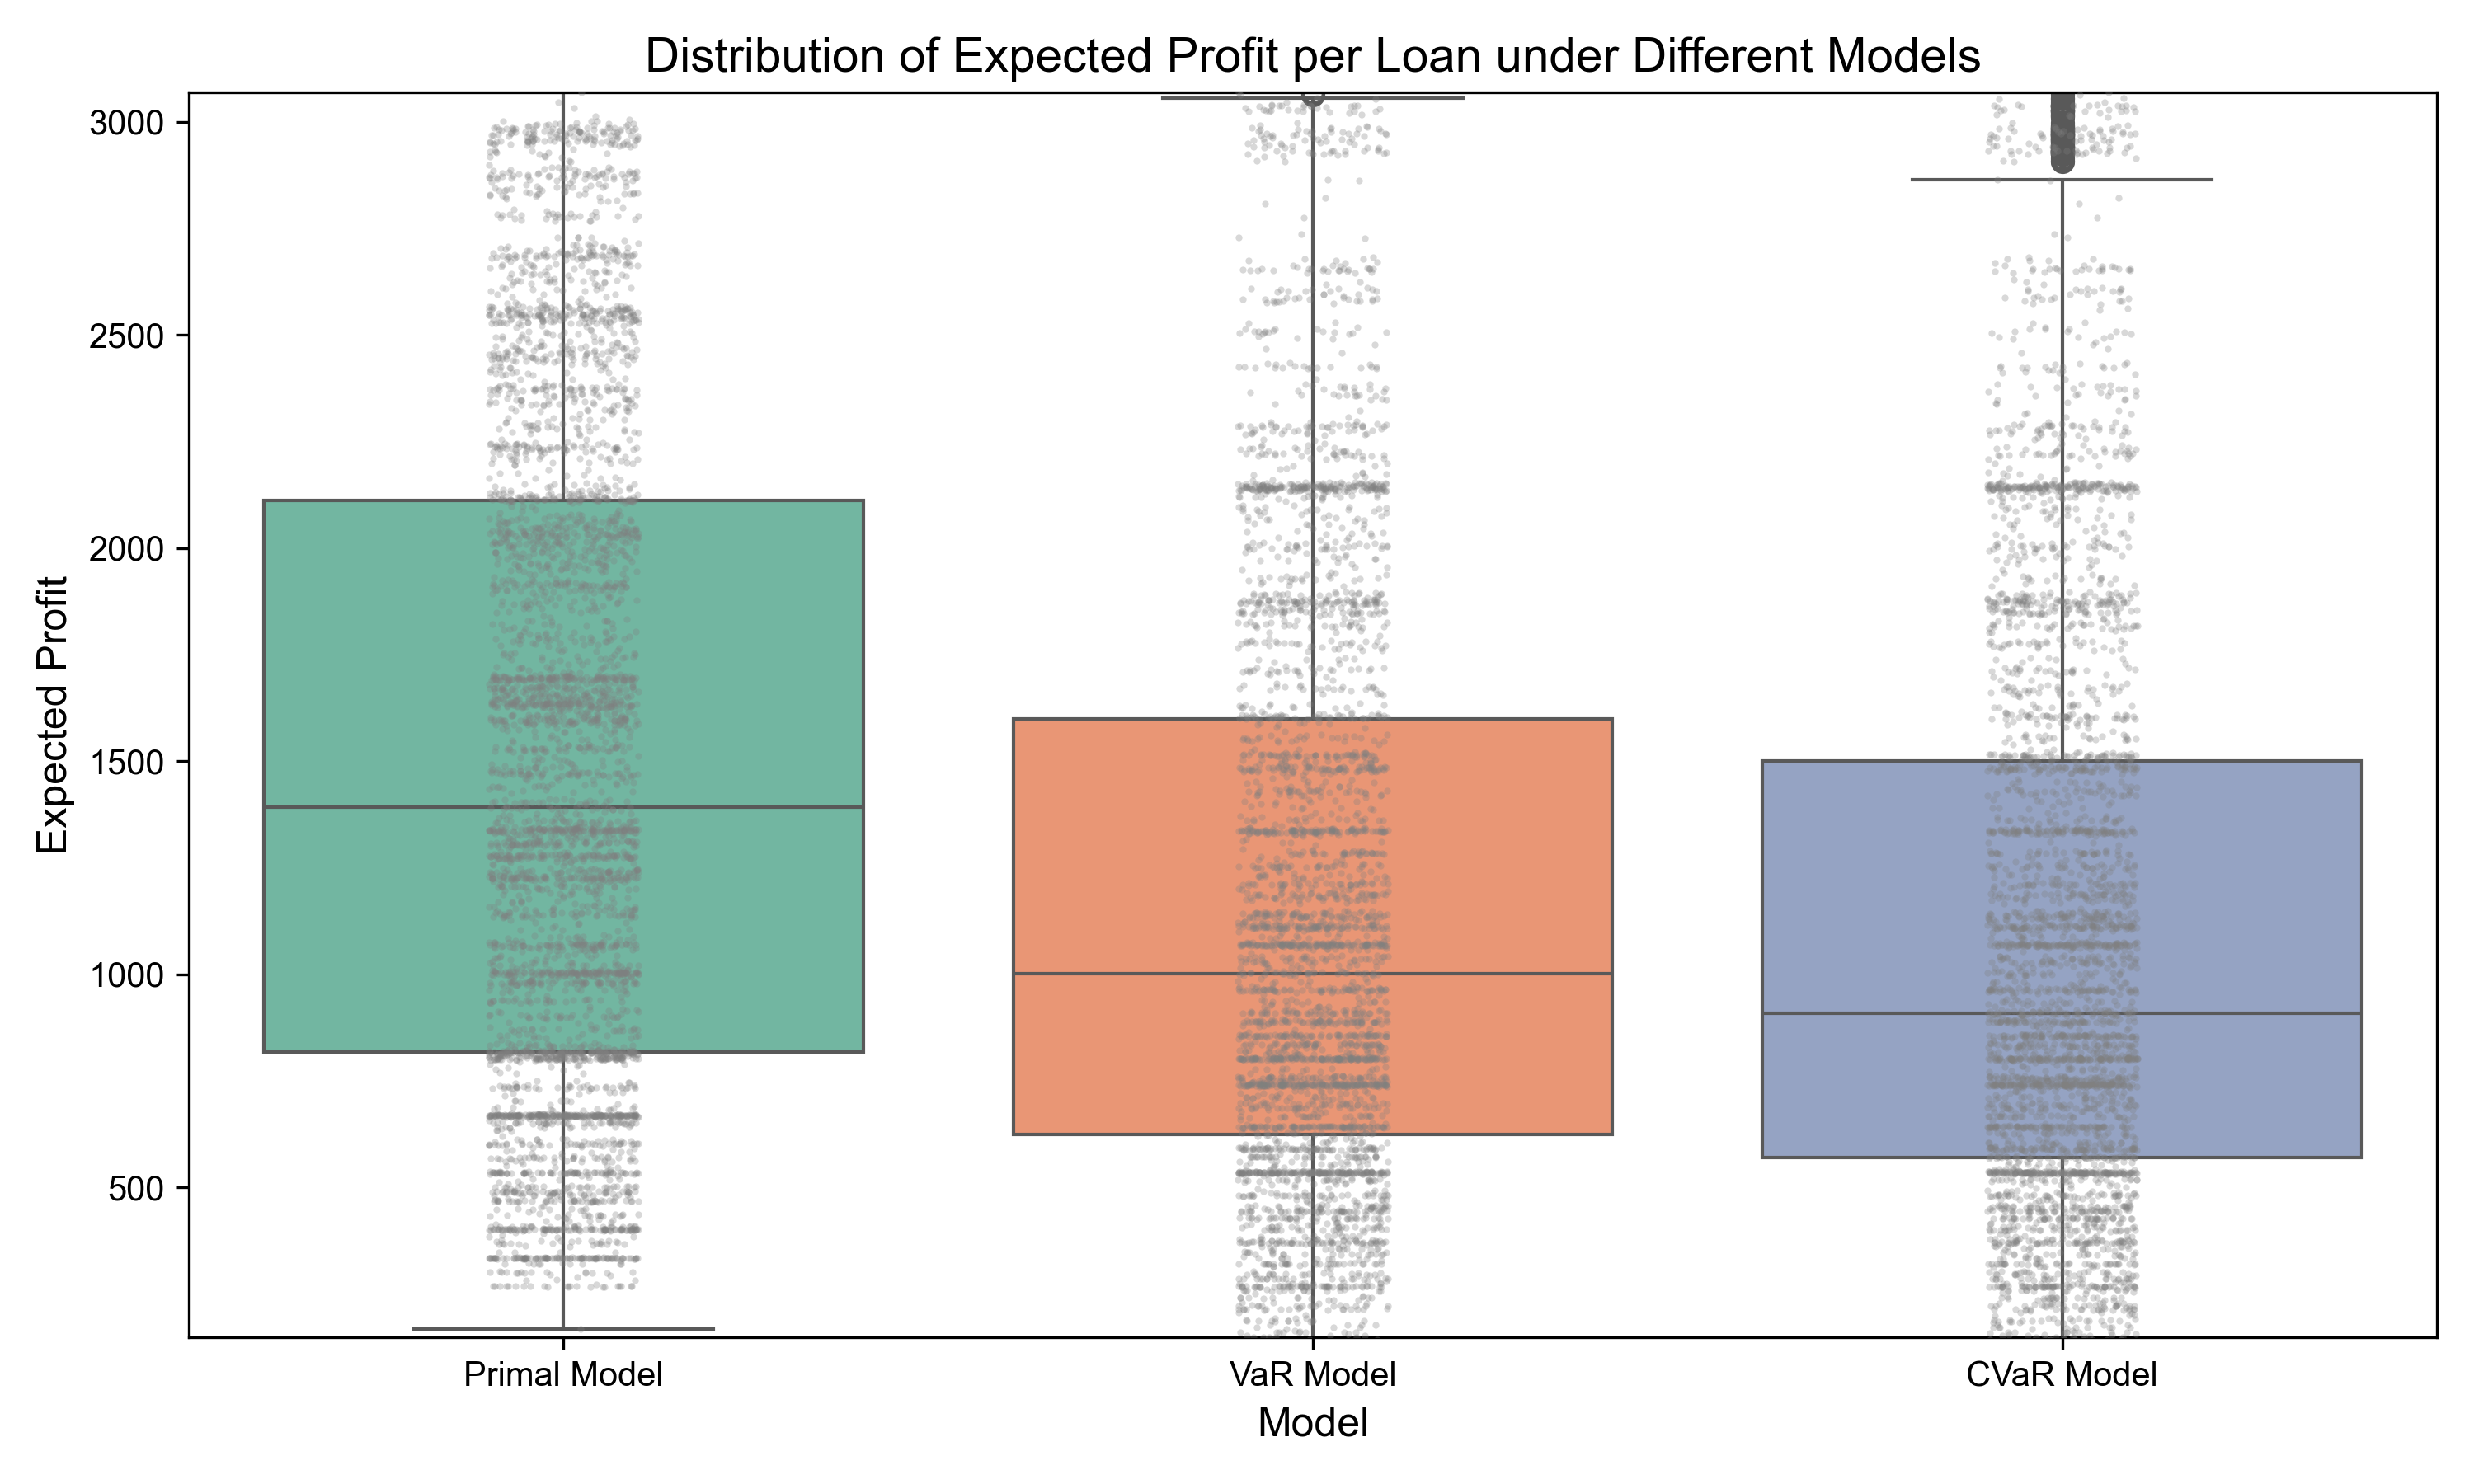
\includegraphics[width=0.48\textwidth]{Figures/model_comparison_expected_profit_boxplot.png}
  \label{fig:expected_profit_boxplot}
}
\subfigure[贷款金额分布]{
  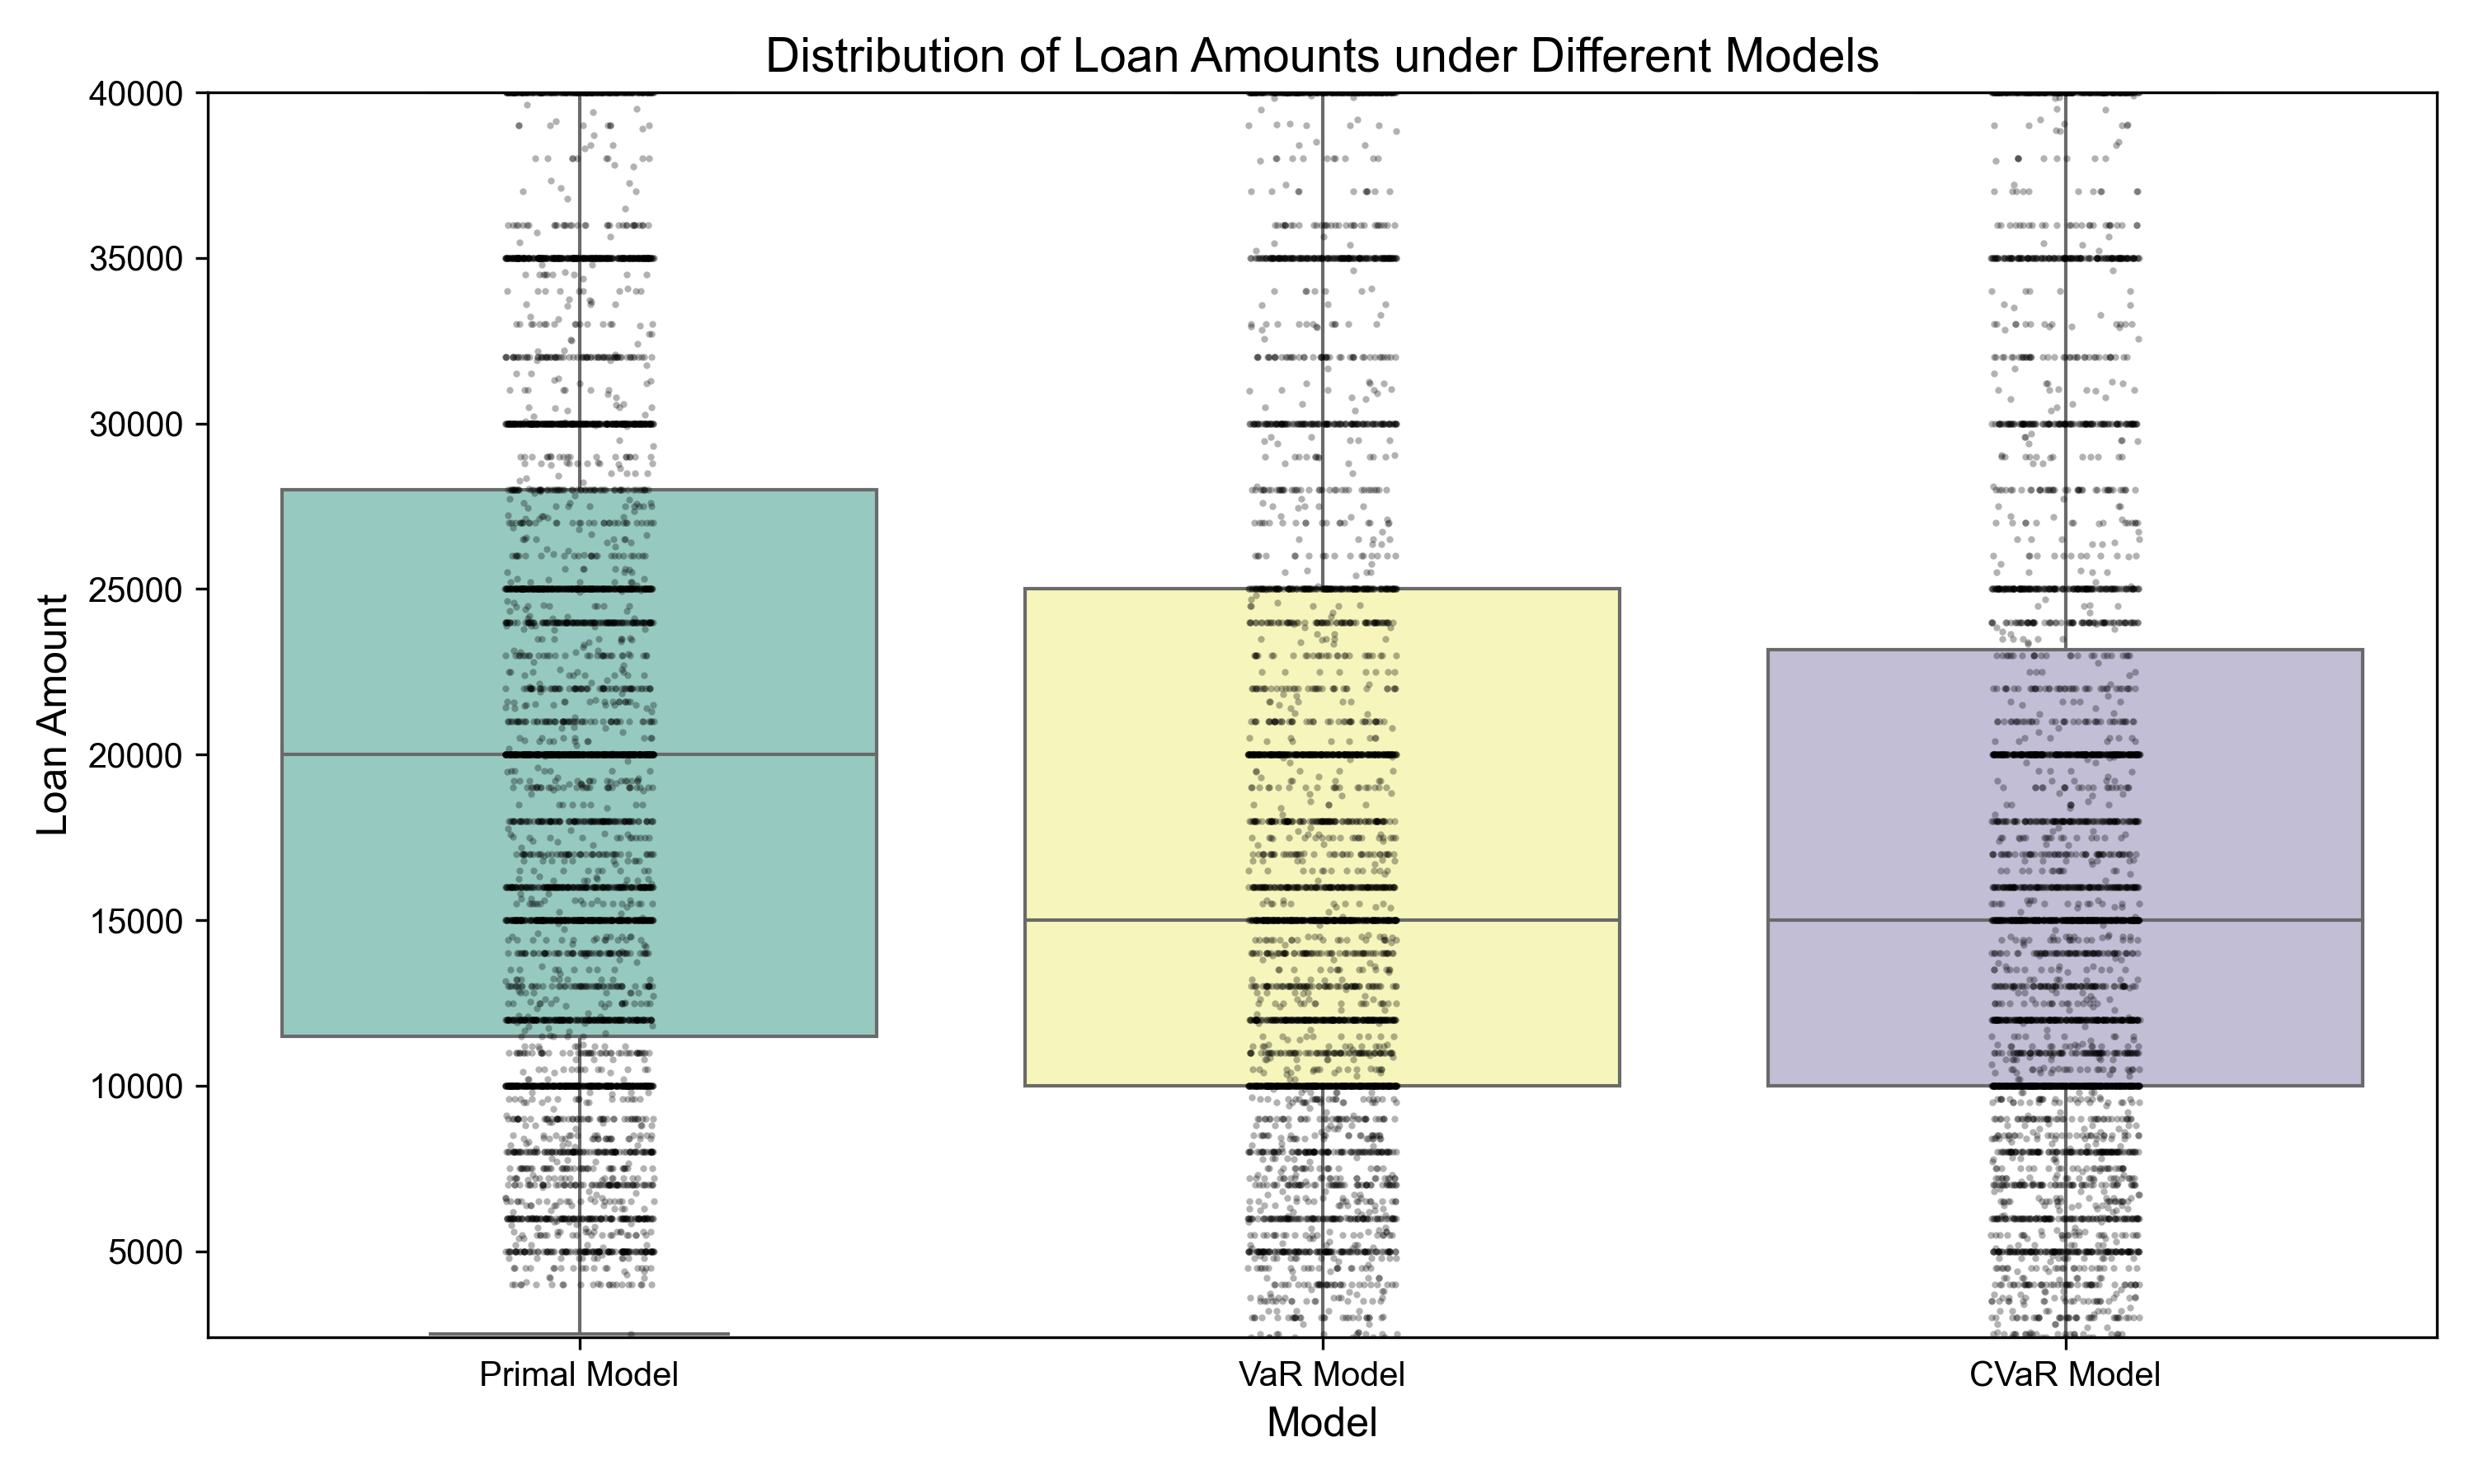
\includegraphics[width=0.48\textwidth]{Figures/model_comparison_loan_amount_boxplot.png}
  \label{fig:loan_amount_boxplot}
}
\caption{三种优化模型下的期望收益与贷款金额分布对比}
\label{fig:boxplot_comparison}
\end{figure}

综上所述,三类模型在贷款筛选策略与风险偏好上体现出显著差异:模型~\ref{eq:main_model} 专注于收益最大化,在缺乏约束的情形下优先选择高利率贷款;模型~\ref{eq:var_model} 在维持一定收益水平的同时,通过 VaR 控制尾部风险事件的发生概率;而模型~\ref{eq:cvar_model} 进一步引入 CVaR 限制,以更严格的方式控制尾部损失均值,体现了其更强的风险规避倾向。上述结果表明,风险约束策略的设置不仅直接影响投资组合的结构和期望收益表现,更深刻地决定了贷款选择的维度分布与风险形态,对金融决策实践具有重要的理论指导与实务启示价值。
\section{结论与启示}
\label{sec:conclusion}

本文基于美国 Lending Club 平台的真实贷款数据,构建了三类贷款投资组合优化模型,分别为期望收益最大化模型、引入 VaR 约束的风险控制模型和引入 CVaR 约束的稳健优化模型。模型考虑了投资预算、贷款信用等级分布、贷款违约概率、极端损失概率与尾部损失均值等关键因素,能够灵活应对不同风险偏好的投资场景。为提升求解效率与解的质量,本文设计了 PSO 与 Gurobi 联合优化框架,在保证计算可行性的基础上,提升了组合的精度与稳健性。

实证结果显示,不同模型在贷款组合选择、期望收益水平与尾部风险控制方面表现出显著差异。期望收益最大化模型在没有设置风险约束的条件下可实现较高的平均回报,但也暴露出更大的尾部风险;VaR 约束模型在控制损失发生概率的前提下,仍保持了相对可观的期望收益水平;CVaR 约束模型则在牺牲部分收益的基础上有效抑制尾部损失,呈现出更强的稳健性。这些结果表明,引入风险约束不仅改变了组合的收益结构,还对贷款选择偏好产生了实质性影响。

从平台管理实践角度出发,研究结果提出了以下启示。首先,应加强风险控制模型的体系化建设,通过引入多维度约束与风险度量(如 VaR、CVaR),提升平台对极端违约风险的识别与应对能力。其次,应根据不同用户画像与资金来源特征,动态设定风险容忍参数,实现收益与风险的平衡优化。此外,风险优化模型的中间变量(如样本 CVaR 或边际 VaR)还可用于贷后监测与风险预警,进一步完善贷中贷后的闭环管理流程。平台亦可基于不同模型的输出结果,设计分层次、差异化的智能投顾方案,为投资者提供更加精细化的信贷资产配置服务。

从模型适用性的角度来看,三类优化模型各具特点。期望收益最大化模型适用于风险容忍度较高、追求高收益的投资者,尤其在宏观市场相对稳定或流动性要求较低的场景下表现良好;VaR 模型在保持收益水平的同时,增强了损失发生概率的可控性,适用于需兼顾监管约束与投资目标的中风险偏好场景;CVaR 模型进一步抑制尾部损失的均值,适合于高安全性需求场景,如养老金投资、机构组合配置或稳健型信贷产品设计。三类模型构成了一个从“收益导向”向“风险导向”递进的优化体系,为信贷投资组合的稳健管理提供了灵活可选的模型架构。

值得注意的是,尽管中国的 P2P 网络借贷平台已在政策主导下于 2020 年前后全面退出市场,但这并不意味着信贷组合优化问题失去了现实基础。相反,当前银行系消费金融公司、小额贷款公司、金融科技助贷平台等新型信贷主体正在承担类似于 P2P 平台的资源配置功能。本文所提出的建模思想、优化框架与风险约束机制,依然适用于这类新型信贷工具的产品设计、风险定价与投资策略制定。尤其是在智能投顾、联合授信、动态授信额度调整等新场景下,VaR/CVaR 等风险约束模型可以作为核心模块嵌入产品逻辑之中,提升系统性风控能力。因此,尽管研究所用数据来自国外 P2P 平台,其结论与方法论对我国金融科技行业在“后 P2P 时代”的信贷创新实践仍具有显著的借鉴意义与理论指导价值。

综上所述,本文在建模层面实现了信贷投资组合从目标函数、约束条件到算法求解的系统性构建;在实证层面揭示了不同风险控制策略对组合结构与收益风险表现的具体影响;在应用层面提供了可迁移、可拓展的优化框架,服务于金融科技时代下多元主体的信贷资源配置需求。未来可进一步考虑引入动态风险视角、多周期投资约束、投资人异质偏好或模型鲁棒性扩展,以增强模型对复杂现实环境的适应性与解释力。


\section*{小组分工}%要出现在目录里面
\addcontentsline{toc}{section}{小组分工}
论文:张璐负责P2P模型建立和借贷背景调研,李晶晶负责违约概率预测,朱冯婧负责模型求解与结果分析。三人共同撰写论文内容。\\
PPT:张璐和李晶晶负责PPT的制作与展示。

\addcontentsline{toc}{section}{参考文献}
\bibliographystyle{unsrtnat} 
\bibliography{ref}
%小组分工


\end{document}
